\section{Hillの式とアロステリック効果}
しかし,実際には式\eqref{normal}に当てはまらない反応が多く確認されている.
生命活動を制御する際には,リガンドの濃度に対して受容体のサイトの占有率がスイッチ的に(ONかOFFかはっきり)応答することが望ましい場合がある\cite{PBoC}.
式\eqref{normal}のような関数では,ON(受容体のサイトが飽和した状態)とOFF(受容体のサイトがガラ空きの状態)の中間の濃度領域が広すぎるのである.

そこで,受容体Yが$n$個の結合サイトを持ち,そのすべてに1個ずつ,リガンドが一斉に結合するような状況を考える.
化学反応式で書くと,
\begin{equation}
  \ce{$n$X + Y <=>[$k$_{on}][$k$_{off}] X_{$n$}Y}
\end{equation}
のようになる.
このときレート方程式は
\begin{equation}
  \dv{t}[\ce{X_{n}Y}] = k_{\mathrm{on}}[\ce{X}]^n[\ce{Y}] - k_{\mathrm{off}}[\ce{X_{n}Y}]
\end{equation}
で与えられる.
これより,定常状態では
\begin{equation}
  \frac{[\ce{X}]^n[\ce{Y}]}{[\ce{X_{n}Y}]} = \frac{k_{\mathrm{off}}}{k_{\mathrm{on}}} = K_d^n
\end{equation}
となる.
ただしここでは$K_d$の$n$乗を解離定数とした.
よって,受容体分子の総濃度を
\begin{equation}
  [\ce{Y_{total}}] = [\ce{Y}] + [\ce{X_{n}Y}]
\end{equation}
と書いて,これを一定と見なすと,受容体の結合サイトの占有率は
\begin{equation}
  p = \frac{[\ce{X_{n}Y}]}{[\ce{Y_{total}}]} = \frac{[\ce{X}]^n}{K_d^n + [\ce{X}]^n} \label{hill}
\end{equation}
となる.

\begin{figure}[htbp]
  \centering
  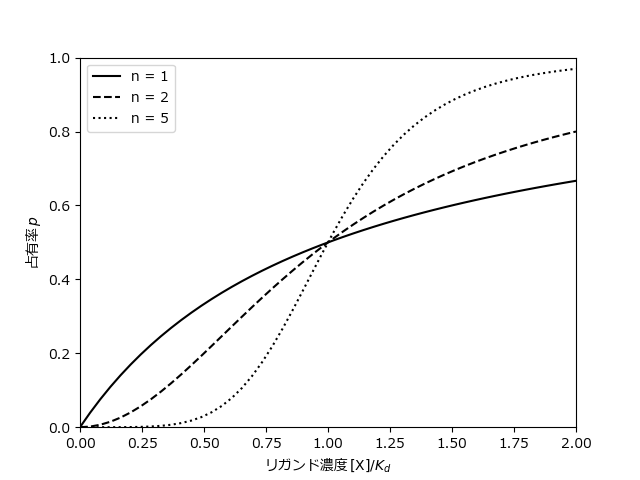
\includegraphics[width=10cm]{hill.png}
  \caption{Hillの式から得られる曲線}
  \label{fig:hill}
\end{figure}

次に式\eqref{hill}を考察する.
$n=1$のときは先ほどの場合とまったく同じだが,$n$を増やすとどうなるだろうか.
計算して確かめると,占有率のグラフはリガンド濃度に対してS字型になることが分かる.
このようなS字型の曲線はシグモイド曲線と呼ばれる.
また,$n$を大きくするほどS字カーブが急峻になることが分かる.
つまり,この$n$を大きくすることで,リガンドの濃度に対するスイッチ的な応答が実現する.

また,Hillの式を導くにあたって,受容体のとりうる状態として$\ce{Y}$と$\ce{X_{$n$}Y}$の二つしか考えなかった.
この状況は,受容体はリガンドが一つ結合した時点で,残りのサイトすべてにリガンドを結合するしかなくなるともいえる.
つまり,リガンドの結合により受容体の状態が変わり,受容体とリガンドが大幅に結合しやすくなったという見方ができる.
このように,受容体のサイトが複数あるとき,あるサイトに何かが結合することで別のサイトでの結合に影響が出ることをアロステリック効果という.


\section{Hillプロット}
また,式\eqref{hill}を変形すると
\begin{equation}
  \qty(\frac{[\ce{X}]}{K_d})^n = \frac{p}{1-p}
\end{equation}
となり,この両辺の対数をとると
\begin{equation}
  \log{\frac{p}{1-p}} = n\qty(\log{[\ce{X}]} - \log{K_d})
\end{equation}
が分かる.
したがって,リガンド濃度$[\ce{X}]$を横軸(x軸)にとり,占有率の高さを表すパラメータ$p/(1-p)$を縦軸(y軸)にとって両対数表示すると,Hillの式に従う場合は直線となる.
また,その直線の傾きは$n$,$p/(1-p)$が1になるときのリガンド濃度は$K_d$となる.
このようなグラフをHillプロットという.
実験結果をもとにこのHillプロットを行うと,測定に使ったリガンドと受容体の振る舞いをHillの式と比較して議論できる.

\begin{figure}[htbp]
  \centering
  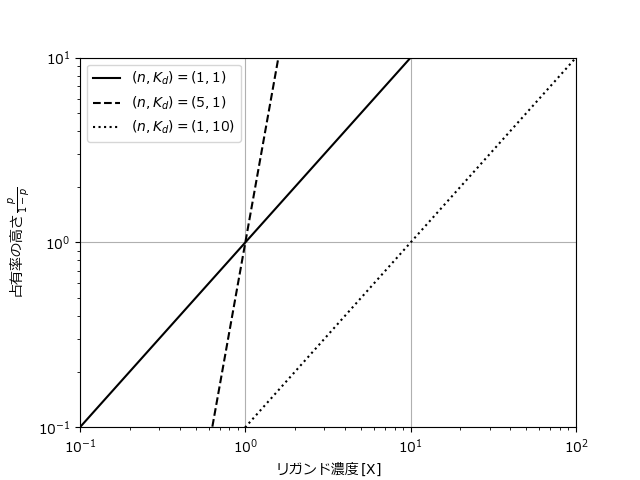
\includegraphics[width=10cm]{hill_plot.png}
  \caption{Hillの式に従う場合のHillプロット}
  \label{fig:hill_plot}
\end{figure}

具体的に受容体としてミオグロビン\footnote{筋肉に含まれる赤色のタンパク質.筋肉が運動して酸素を消費するときに備えて,普段は酸素を蓄える働きをする.}を,リガンドとして酸素を考える.
この場合にHillプロットを行うと,ミオグロビンのサイトの占有率は直線的になり(Hillの式に従い),$n=1$と求まる.
つまり,ミオグロビンは「最も単純なモデル」に従う受容体である.
一方で,受容体としてミオグロビンの代わりにヘモグロビン\footnote{赤血球に含まれる赤色のタンパク質.肺で受け取った酸素を全身に運搬する役割を担う.ミオグロビンは酸素の受け取り手の一つである.ちなみに,魚の赤身と白身の区別はヘモグロビンとミオグロビンの含有率に由来する.赤身の魚は長時間活発に泳ぐことができるが,これはヘモグロビンやミオグロビンが多いことで酸素を効率よく筋肉に回せるからである\cite{akami}.}を考えると,今度はHillプロットが直線的にならない部分が現れる.
それでもHillの式でフィッティングして$n$を求めると,$n=2$と$n=3$の間の非整数値となってしまう.
つまり,ヘモグロビンと酸素の結合はHillの式ではうまく説明できない.